%% LaTeX template for BSc Computing for Games final year project dissertations
%% by Edward Powley
%% Games Academy, Falmouth University, UK

%% Based on:
%% bare_jrnl.tex
%% V1.4b
%% 2015/08/26
%% by Michael Shell
%% see http://www.michaelshell.org/
%% for current contact information.
%%
%% This is a skeleton file demonstrating the use of IEEEtran.cls
%% (requires IEEEtran.cls version 1.8b or later) with an IEEE
%% journal paper.
%%
%% Support sites:
%% http://www.michaelshell.org/tex/ieeetran/
%% http://www.ctan.org/pkg/ieeetran
%% and
%% http://www.ieee.org/

%%*************************************************************************
%% Legal Notice:
%% This code is offered as-is without any warranty either expressed or
%% implied; without even the implied warranty of MERCHANTABILITY or
%% FITNESS FOR A PARTICULAR PURPOSE! 
%% User assumes all risk.
%% In no event shall the IEEE or any contributor to this code be liable for
%% any damages or losses, including, but not limited to, incidental,
%% consequential, or any other damages, resulting from the use or misuse
%% of any information contained here.
%%
%% All comments are the opinions of their respective authors and are not
%% necessarily endorsed by the IEEE.
%%
%% This work is distributed under the LaTeX Project Public License (LPPL)
%% ( http://www.latex-project.org/ ) version 1.3, and may be freely used,
%% distributed and modified. A copy of the LPPL, version 1.3, is included
%% in the base LaTeX documentation of all distributions of LaTeX released
%% 2003/12/01 or later.
%% Retain all contribution notices and credits.
%% ** Modified files should be clearly indicated as such, including  **
%% ** renaming them and changing author support contact information. **
%%*************************************************************************


\documentclass[journal]{IEEEtran}

\usepackage{listings}
\usepackage{graphicx}
% Insert additional usepackage commands here
\graphicspath{ {Figures/} }
\usepackage{float}
%\usepackage{wrapfig}
\usepackage{amsmath}
%\usepackage[linesnumbered,ruled]{algorithm2e}
\usepackage{xargs}                      % Use more than one optional parameter in a new commands
\usepackage[pdftex,dvipsnames]{xcolor}  % Coloured text etc.
\usepackage{todonotes}
\usepackage{algpseudocode}
\usepackage{algorithm}% http://ctan.org/pkg/algorithms

%\usepackage[figuresonly,nolists,nomarkers]{endfloat}
%\renewcommand{\processdelayedfloats}

\begin{document}
	%
	% paper title
	% Titles are generally capitalized except for words such as a, an, and, as,
	% at, but, by, for, in, nor, of, on, or, the, to and up, which are usually
	% not capitalized unless they are the first or last word of the title.
	% Linebreaks \\ can be used within to get better formatting as desired.
	% Do not put math or special symbols in the title.
	\title{ How Does Visualising Path-finding in an NPC Affect How Players Explore a Game Level?}
	%
	%
	% author name
	\author{Madeleine Kay}
	
	% The paper headers -- please do not change these, but uncomment one of them as appropriate
	% Uncomment this one for COMP320
	%\markboth{COMP320: Research Review and Proposal}{COMP320: Research Review and Proposal}
	% Uncomment this one for COMP360
	\markboth{COMP360: Dissertation}{COMP360: Dissertation}
	
	% make the title area
	\maketitle
	
	% As a general rule, do not put math, special symbols or citations
	% in the abstract or keywords.
	\begin{abstract}
		% Opening: 
		This paper looks at the use of path-finding and~\textit{Artificial Intelligence} (AI) visualisation in digital games.   Specifically at the use of foregrounding AI and the visualisation of path-finding. 
		%    Challenge: 
		While previous papers have researched AI visualisation and how to achieve it there does not appear to be many papers on the field of visualising AI in video games. There has been research into the visualisation of path-finding. However, the focus was most commonly on the use of visualisation in game design. 
		% Action: 
		This paper looks at visualising various methods of path-finding on enemy NPCs in a 3D Metroidvania game developed in Unity.
		%Resolution:
		The results found a number of cases where player exploration was effected by either a change in path-finding method or whether the path-finding is visualised. This suggests that these factors effect player exploration and could be taken into account when designing games.
		
	\end{abstract}
	
	\section{Introduction} \label{introduction}
	\IEEEPARstart{T}{his} project looks at visualising the path-finding of an enemy~\textit{Non Player Character} (NPC) using~\textit{Rapidly-exploring Random Tree} (RRT) path-finding.  Figure~\ref{KuffnerRRT} shows an example of RRT path-finding. Here the RRT explores the area and then draws a path along the tree between the start and the goal nodes~\cite{Kuffner2000}. 
	
	This paper looks at visualising the tree produced by RRT and the process taken to produce it. The visualisation is around an enemy NPC. This allows the players to see where the enemy NPC is going and where it could go. 
	
	Implementation of the visualisation was developed in a level of a 3D game made in Unity 5.6\footnote[1]{Unity 5.6 Available: https://unity3d.com/get-unity/download/archive}. Logging tools in the play-testing software export the amount of time the players spent in a level and what percent of the level they explored. Analysis of this data found that only two cases had an effect on player exploration. These two were the visualisation of the Unity navmeshes had a negative correlation with the amount of the level explored and the use of RRT path-finding increasing the amount of the level explored. This is analysed in more detail in section \ref{Analysis}.
	
	Previous papers have researched visualising \textit{Artificial Intelligence} (AI) and foregrounding AI. However, there is little on what effect this has on how the players explore the game.
	The research question proposed in this project is: how does visualising RRT path-finding in an NPC affect how a player explores a game level?
	
	\section{Roadmap}
	Section~\ref{RelatedWork} is a review of the literature on existing relevant work. The areas reviewed are A* path-finding, RRT path-finding, path-finding, foregrounding AI and exploring game environments. 
	Section~\ref{methodology} details the methodology used in the experiments in this study. Section~\ref{softdev} details the development of the software used for the experiments in this study.
	Section~\ref{datacollection} details the data collected and how it was filtered and section~\ref{Analysis} looks at the analysis of this data and what the results infer. Section~\ref{PotentialIssues} details the potential issues and ways to address them in future work. Section~\ref{FutureWork} looks at future research that could be done on this subject. 
	
	\section{Related Work} \label{RelatedWork}
	The focus of this paper is on path-finding so that is the main focus of the literature review. The path-finding methods looked at are A* path-finding in section~\ref{A*PF} and RRT path-finding in section~\ref{RRTadnPathfinding}.  Section~\ref{VisualisingAI} looks at foregrounding and visualising AI. While there is research on AI visualisation there is a lack of it for digital games and what research is on games often focuses on game development and level design as can be seen in section~\ref{VisualisingAI}. 
	This literature review shows that while there are many papers on AI visualisation there are few on AI visualisation in digital games and many of the ones on games are on visualising AI to aid development, not for the end user.     
	
	\subsection{A* Path-finding} \label{A*PF}
	A* path-finding is widely used in both robotics and digital games~\cite{Algfoor2015}. In games, A* appears to be the most commonly used path-finding algorithm~\cite{Algfoor2015}.
	
	Hart~\textit{et al}~\cite{Hart1968} first proposed A* path-finding in 1968 as an improvement on Dijkstra's algorithm. A* aims to expand the fewest nodes possible to minimise the cost of the path where the cost is the distance between the start and goal nodes. Figure~\ref{A*Pseudo} shows pseudo-code for implementing A*. 
	
	\begin{figure}[h]
		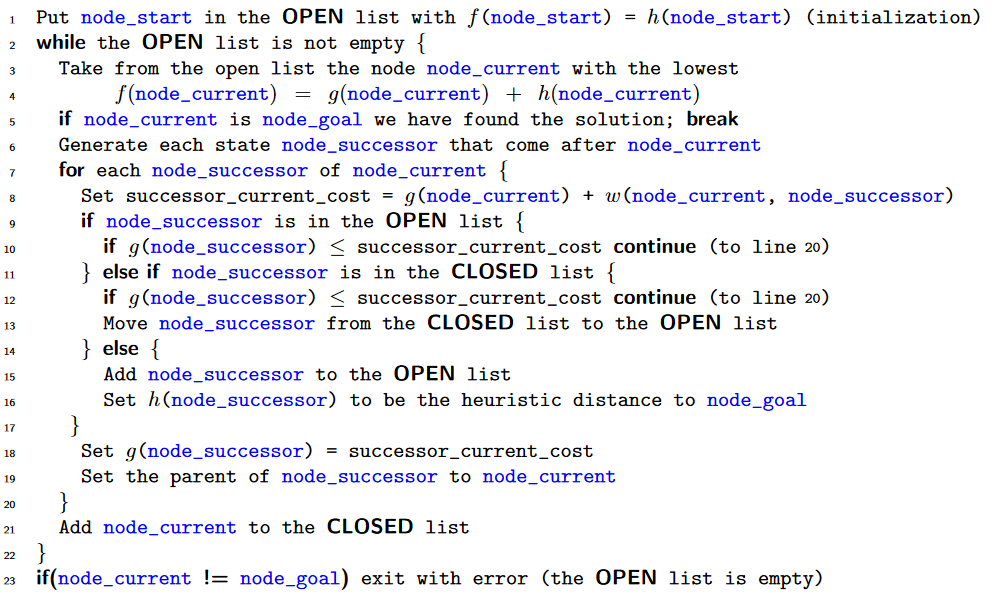
\includegraphics[width=1.0\linewidth]{APseudocode.png}
		\caption{Pseudo-code for A* path-finding~\cite{Hart1968}~\cite{pseudocode:A*}.}
		\label{A*Pseudo}
	\end{figure} 
	
	Algfoor~\textit{et al}~\cite{Algfoor2015} surveyed numerous papers on path-finding. Their focus was on the use of different grid shapes in path-finding and the numerous algorithms available~\cite{Algfoor2015}. The most popular being the A* algorithm for use in both digital games and robotics. They surveyed many grid types and gave the advantages of each. 
	
	Nash~\textit{et al}~\cite{Nash2007} say that A* cannot always find the true shortest path as it is limited to the grid. The shortest path can be found A* with post-smoothing paths or by using A* variants such as Theta*~\cite{Nash2007, Firmansyah2016}. Theta* expands on A* as it allows for all edges and angles in the grid to be used. Therefore, a path with a more optimal distance can be found.
	
	While their focus is on Android games Firmansyah~\textit{et al}~\cite{Firmansyah2016} compared A* with Theta*. They found that performed similarly time wise. However, A* produced a path with fewer nodes expanded and Theta* produced a shorter path. 
	
	Hu~\textit{et al}~\cite{Hu2012} propose an implementation of A* path-finding in the Unity engine, the engine used in this project.  While their implementation is in an older version Unity the implementation in Unity 5.6 should still be similar. A further paper on path-finding is Wang and Lu's~\cite{wang2012} paper which looks at path-finding in a 3-Dimensional environment. While again they were using A* they look at using A* in 3D and suggest using nodes instead of a grid.
	
	Tremblay~\textit{et al}~\cite{Tremblay2014} look at the use of path-finding algorithms in level design. They compared 2-Dimensional A*, 3-Dimensional A*, RRT using A* for motion planning, RRT using~\textit{Monte Carlo Tree Search} (MCTS) and MCTS alone. 2-Dimensional A* consistently gave the fastest result with the highest success rate. As this was for game level design instead of gameplay they ran the algorithms 1000 times on high specification computers. 
	
	For this project, the algorithm will only be run once as it is being used at runtime in the game instead of in the game design stage that Tremblay~\textit{et al}~\cite{Tremblay2014} tested in. As A* has a 100 percent chance of finding the shortest path this should not cause an issue. 
	
	\subsection{RRT and Path-finding} \label{RRTadnPathfinding}
	RRTs are a search method used more in robotics than in digital games~\cite{LaValle1998, Kuffner2000}. Kuffner and LaValle~\cite{Kuffner2000} first proposed RRT in 2000. They intended to produce a random algorithm more efficient than the other search algorithms available at the time.  Figure~\ref{KuffnerRRT} shows Kuffner and LaValle's~\cite{Kuffner2000} RRT Path Planner. Path Planner is a variant of RRT which has the intended use of finding paths from the generated tree.
	
	\begin{figure}[h]
		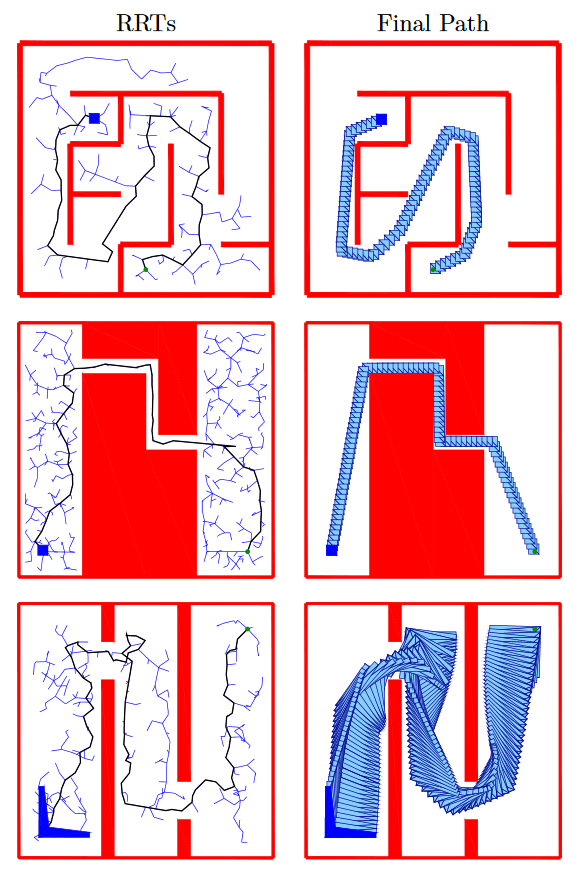
\includegraphics[width=1.0\linewidth]{KuffnerRRT.png}
		\caption{ Kuffner and LaValle's RRT path planner building a tree and plotting a path through it~\cite{Kuffner2000}.}
		\label{KuffnerRRT}
	\end{figure} 
	
	\begin{algorithm}
		\begin{algorithmic}
			\State \hrulefill 
			\State \textbf{ BUILD\_RRT($q$init)}
			\State $T$.init($q.init$)
			\For{$k = 1$ to $K$} 
			\State $q$rand $ \gets  RANDOM$\_$CONFIG() $
			\State EXTEND ($T$, $q$rand)
			\EndFor
			\State \hrulefill
			\State \hrulefill 
			\State \textbf{EXTEND($T$, q)}
			\State $q$near $ \gets $ NEAREST\_NEIGHBOR($q, T$);
			\If {NEW\_CONFIG($q, qnear, qnew$)}
			\State $T$.add\_vertex($q$new);
			\State $T$.add\_edge(qnear, qnew);
			\If {$q$new = $q$}
			\State Return $Reached$;
			\Else
			\State  Return $Advanced$;
			\EndIf
			\State Return $Trapped$
			\EndIf
			\State \hrulefill 
		\end{algorithmic}
		\caption{RRT Pseudo Code}
		\label{RRTPseudocode}
	\end{algorithm}
	
	The process for RRT involves the random placement of nodes. A parent is then selected by finding the closest pre-existing node~\cite{Kuffner2000}. Algorithm~\ref{RRTPseudocode} shows the pseudo-code for the RRT algorithm. 
	
	RRTs goal is to find a path between two points with no collisions.  The path found may not be the optimal path though~\cite{Kuffner2000, Karaman2011}. Karaman and Sertac~\cite{karaman2010} say that the chance of RRT finding an optimal path is very unlikely~\cite{karaman2010, Tremblay2014}. Where A* is guaranteed to find the shortest path as seen in section~\ref{A*PF}, RRT is unlikely to find the shortest path and may not even find a path at all.  
	Karaman~\textit{et al} propose a variant of RRT called RRT*. RRT* starts the same as RRT, however, when a new node has to choose a parent node instead of selecting the nearest node it evaluates the cost of the nodes in regards to reaching its goal. Each iteration re-evaluates the parent nodes to reduce the cost. Rewiring of the tree happens when a lower cost path is found.
	
	\subsection{Path-finding} \label{Pathfinding}
	Bauer and Popovic~\cite{bauer2012} use RRT for level design in digital games. Like other papers mentioned in section~\ref{VisualisingAI}, they visualise the data to aid users~\cite{bauer2012, Haworth2010}. This data visualisation is for use in game development to aid game developers or to analyse procedurally generated levels. 
	
	\begin{figure}[h]
		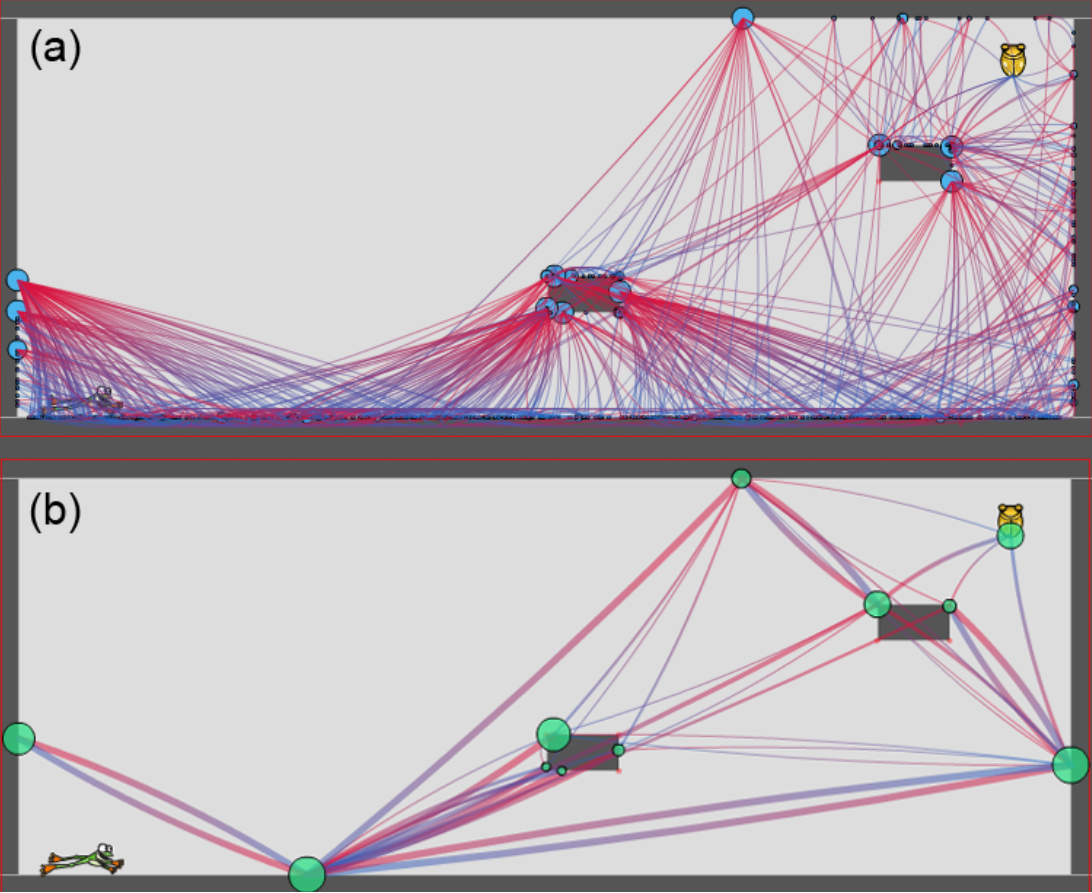
\includegraphics[width=1.0\linewidth]{BauerRRT.png}
		\caption{ Bauer~\textit{et al}'s\cite{bauer2012} graph-based representation of RRT with and without clustering.}
		\label{BauerRRT}
	\end{figure} 
	
	Their focus is on level design, not game-play. They propose a tool that analyses a level generated by PCG or a level designer. They then use RRT to calculate possible routes the player could take when playing.  Figure~\ref{BauerRRT} shows the output of the tool once it has been run on a basic level design.  The first image, image a, may be difficult to read. So, they make use of Dongen's method for graph clustering to make the output more legible as shown in the second image, image b~\cite{bauer2012, Dongen2001}.  
	
	The focus of this project is on a similar type of visualisation but running in the game instead of during the game development. Therefore, there is a need for a similar technique to cluster the output of RRT. This should make the visualisation more useful as it should aid the player in a way that they can look at the visualisation and interpret what the NPC is going to do. 
	
	Mendonça~\textit{et al}~\cite{Mendonça2015} look at path-finding both in robotics and digital games. Their focus is on stealth path-finding in games and applying that to robotics. Like RRT, the methods they propose do not necessarily find the shortest path~\cite{karaman2010, Mendonça2015}. Instead, they try to find the path where the agent spends most of the time in cover. They generate custom~\textit{navigation meshes} (navmeshes). Then they assign a weight to each polygon in the navmesh depending on how close it is to being behind cover. 
	
	As Mendonça~\textit{et al}~\cite{Mendonça2015} use path-finding to find a stealth orientated path. The path with the optimal distance may not always be the path with the lowest cost in relation to the AI agent being in cover. Therefore, a requirement might not always be the shortest path. 
	
	Tremblay~\textit{et al}~\cite{Tremblay2013}, like Bauer and Popovic~\cite{bauer2012}, also use RRT visualisations to aid level design. They use RRT to visualise possible moves the player could make. Then they use clustering to make the results less cumbersome to the user~\cite{Tremblay2013}. Similar to Mendonça~\textit{et al}~\cite{Mendonça2015}, they focus on designing stealth games and finding stealth orientated paths in the game levels~\cite{Tremblay2013}.   Figure~\ref{TremblayHeatMap} shows the basic level design they used with three areas for the AI agent to take cover. This allows level designers to see where players are likely to go and adjust the level design accordingly~\cite{Tremblay2013}.  The use of RRT, in this case, is because it is flexible and inexpensive. Also, its random nature allows for the mimicking of a wider range of player behaviours~\cite{Tremblay2013}. 
	
	This project uses RRT but not for reflecting player behaviour.  Instead, its use is for creating a visualisation that fits with the game and that may be interesting for the player to interact with. A path that is interesting to play with is more important in this project than a path with an optimal distance. There is then a comparison between a visualisation of the Unity navmeshes against the RRT visualisation.
	
	While the use of RRT to find a stealth orientated paths is different to its use in this project a potential problem is that Tremblay~\textit{et al}'s results showed that the chances of their RRT implementation finding a path decreased as the grid size increased. It also decreased as the number of attempts decreased as shown in Figure~\ref{TremblayRRT}.  This suggests that a potential issue with RRT is that it may not always find a path.
	
	\begin{figure}[h]
		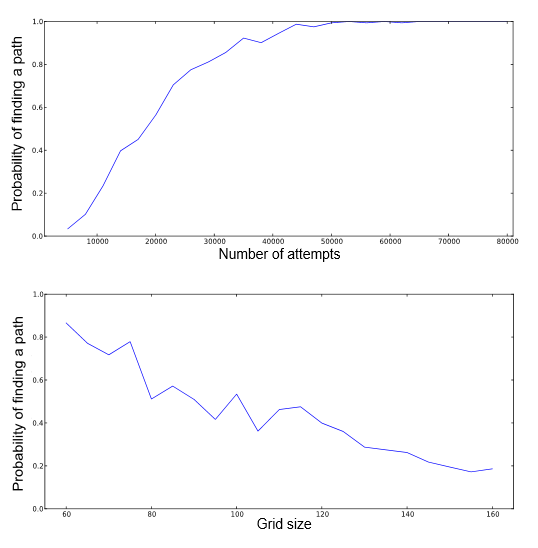
\includegraphics[width=1.0\linewidth]{Tremblay2013.png}
		\caption{ Performance analysis of Tremblay~\textit{et al}'s~\cite{Tremblay2013} RRT when running on a Metal Gear Solid level~\cite{game:MetalGearSolid}.}
		\label{TremblayRRT}
	\end{figure} 
	
	\begin{figure}[h]
		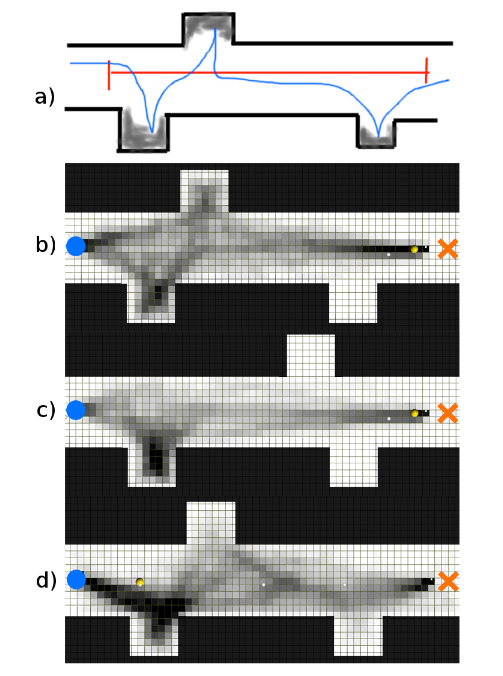
\includegraphics[width=1.0\linewidth]{TremblayHeatMap.png}
		\caption{Heat maps of a single level where the design has been changed each time~\cite{Tremblay2013}.}
		\label{TremblayHeatMap}
	\end{figure} 
	
	Tremblay~\textit{et al}~\cite{Tremblay2014} again look at the use of search algorithms for use in game development. This work builds on their 2013 paper on RRT in stealth games. As previously mentioned in section~\ref{A*PF} they look at the use of A*, MCTS and RRT to visualise player behaviour in platform games similar to Bauer ~\cite{Tremblay2014}~\cite{bauer2012}.  RRT is limited to drawing straight lines between the nodes, as straight lines are not always possible in RRT Tremblay~\textit{et al}~\cite{Tremblay2014} also use either A* or MCTS to find a path to the node and ensure that it is reachable.
	While A* is consistently fast with high success rates, RRT has varying results. RRT using MCTS for motion planning varied between 35 and 84 percent success rates and had the longest run times. In comparison, RRT with A* motion planning consistently had a success rate of over 60 percent. However, the run times for this combination varied. 
	Both of Tremblay~\textit{et al}'s~\cite{Tremblay2014, Tremblay2013} papers showed that a potential issue with the use of RRT is that it may not find a path. Both papers ran RRT combinations over 1000 times. In comparison, this paper runs RRT at runtime and only runs the algorithm once unless an RRT variant such as RRT* is used. If a path is not found a tree is still produced and visualised so may still influence players.
	
	Section~\ref{VisualisingAI} looks at Third Eye Crime in more detail for its use of AI visualisation. However, it also uses visualisation of enemy paths as an important mechanic~\cite{Isla2014, game:ThirdEyeCrime}.  Isla~\cite{Isla2014} uses Occupancy Maps to show where the enemy NPC thinks the player could be. Occupancy or Influence Maps do not produce a path instead they show the probability of the player being in different locations across the map~\cite{Isla2014, Miles2006}. Isla used Occupancy Maps to show where the enemy AI thinks the player currently is. The enemy then moves to investigate that area reducing the probability of the player being there.  Similarly, Miles and Louis~\cite{Miles2006} also used influence maps. While their example is specific to~\textit{Real Time Strategy} (RTS) games, like Isla they used Occupancy Maps.  They used them as a base for A* path-finding instead of A* using the map itself for path-finding.
	
	
	\subsection{Foregrounding and Visualising AI} \label{VisualisingAI}
	Most modern digital games make use of AI.  However, it is rarely foregrounded or visualised in those games. Treanor~\textit{et al}~\cite{treanor2015} say that often the design of AI in games is to fit the game and complement gameplay. These AI are supporting the gameplay rather than being central to it.
	
	Treanor~\textit{et al}~\cite{treanor2015} surveyed many games that foreground or visualise AI in different ways.   From this, they propose a series of design patterns for foregrounding AI in digital games. 
	The two design patterns relevant to this project are ``AI as a Villain" and ``AI is Visualised".  They describe the first pattern as having the AI try to not outright defeat the player. Instead, it is designed to create an experience like in the game Alien Isolation~\cite{treanor2015, game:AlienIsolation}.  In Alien Isolation the enemy AI hunts the player. This is foregrounding as the player must observe the AI and learn how to avoid it. There is also some visualisation as the player has a scanner that informs them of the enemy's position. 
	
	This paper uses the ``AI as a villain" pattern as each enemy NPC has their path-finding visualised around them. The players can consider this when exploring a level so they do not get attacked by the enemy. The use of this pattern also aims to have an NPC that creates an experience rather than one that always finds the player, similar to Alien Isolation~\cite{game:AlienIsolation,treanor2015}. While the player likely does not want to be caught by the enemy NPC they may want it to chase them so they can learn its patterns or lead it away from other enemies to make it easier to attack. 
	
	The second relevant design pattern is ``AI is Visualised".  This is where there is a visual representation of the AI's state or decision making in the game~\cite{treanor2015}. Most games hide this from the player but this design pattern visualises it making it mechanic.  
	The example given by Treanor~\textit{et al}~\cite{treanor2015} is the game Third Eye Crime.  Third Eye Crime is a game that follows the ``AI is Visualised" design pattern~\cite{Isla2014, game:ThirdEyeCrime}. The game uses probabilistic object tracking through Occupancy Maps. The game uses Occupancy Maps to display where the enemy thinks the player could be on the map, as can be seen in figure~\ref{image:ThirdEyeCrime}. As the enemy moves around the map it removes areas where the player is not from the Occupancy Map~\cite{Isla2014}.  Generally, stealth games involve avoiding enemies.  This design encourages the player to trigger the mechanic, allowing them to use the visualisation to mislead and avoid the enemy~\cite{Isla2014, game:ThirdEyeCrime}. 
	
	\begin{figure}[h]
		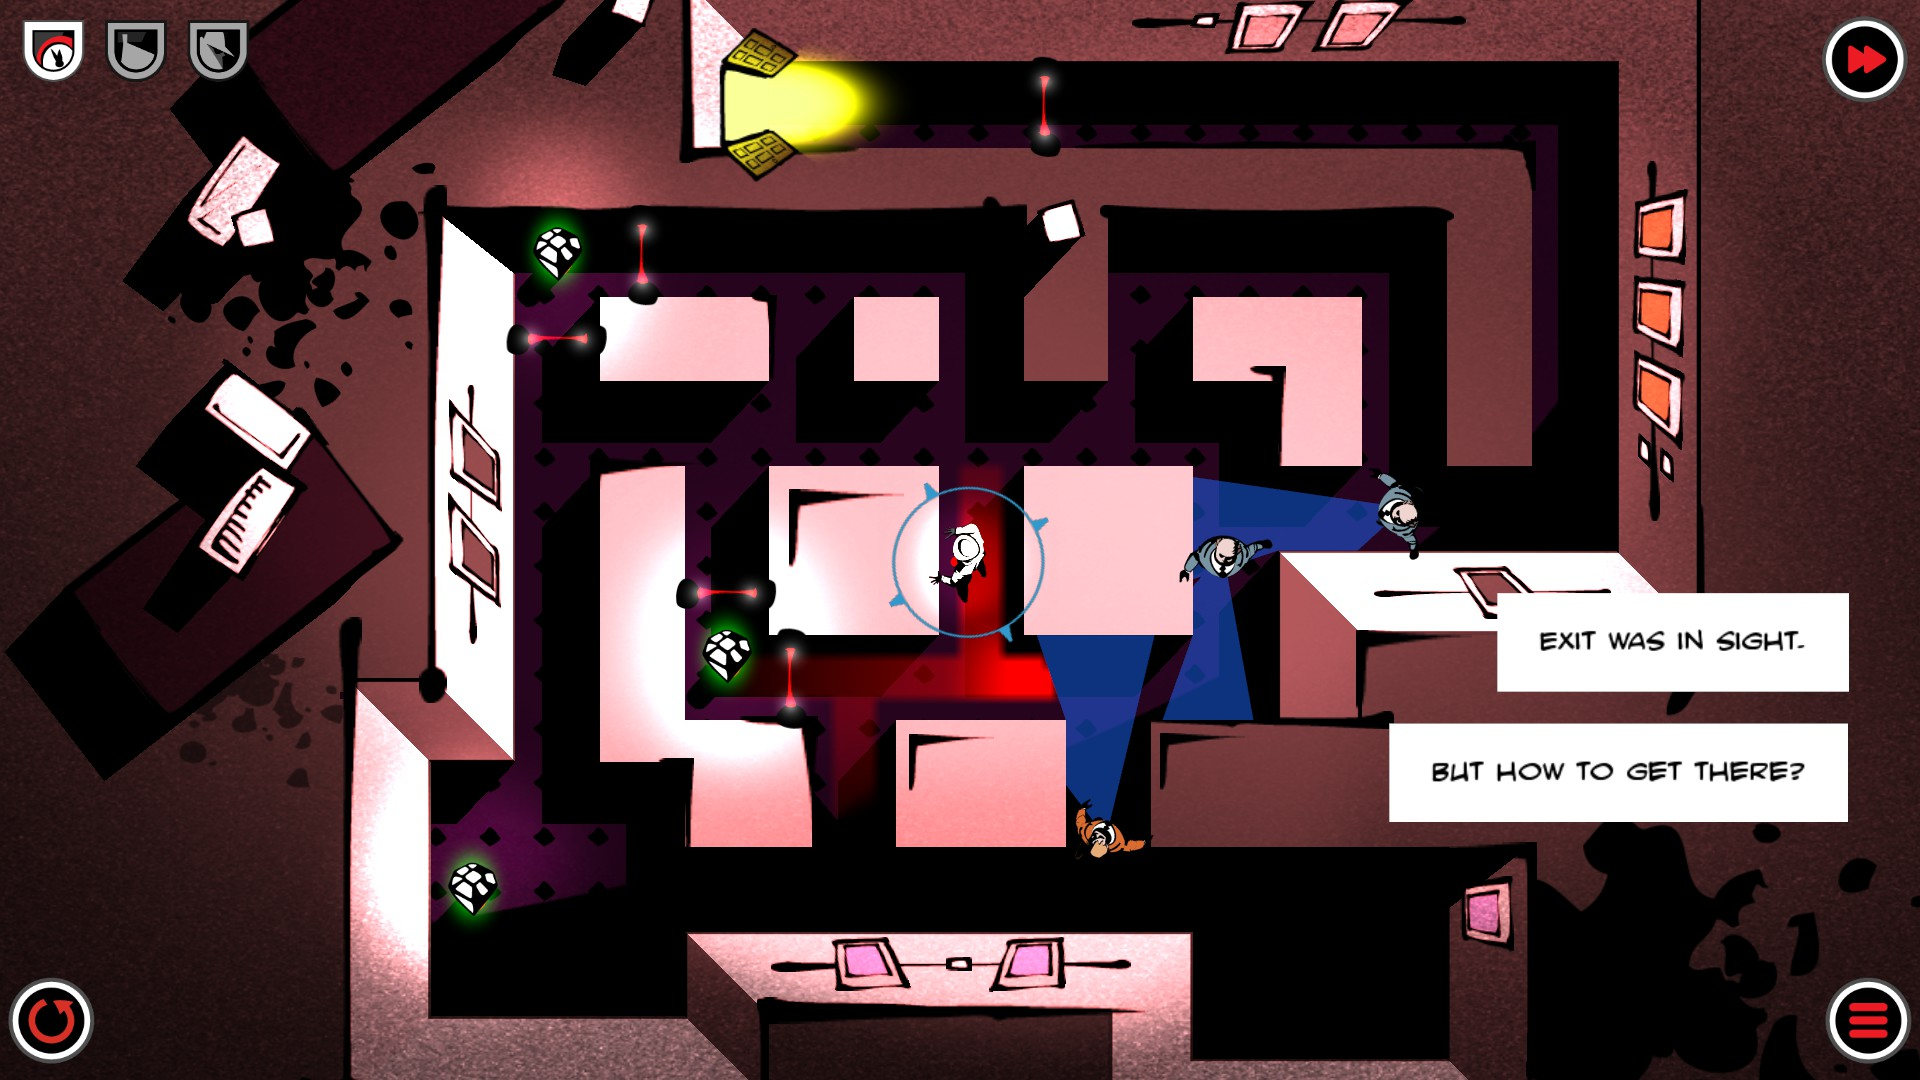
\includegraphics[width=1.0\linewidth]{ThirdEyeCrime.jpg}
		\caption{ A screen-shot from Third Eye Crime~\cite{game:ThirdEyeCrime}.}
		\label{image:ThirdEyeCrime}
	\end{figure}  
	
	This pattern is relevant to this project as the enemy NPCs have RRT path-finding visualised around it allowing the player to see where the enemy is searching and decide how to overcome or outsmart it.
	
	% Visualising in general
	While Haworth~\textit{et al}~\cite{Haworth2010} do not visualise an AI decision-making process they do visualise the possible decisions available to the player in a game on a tree structure.   They research visualising decision trees in a game to see what effect it had on gameplay and the analytical reasoning of children.  
	Their study does not come to any definite conclusions. However, their results suggest that the trees aided players as in the later levels of the game the children without the visualised decision tree struggled to beat the game. However, they noted this could also be due to unbalanced difficulty in the later levels. This makes the usefulness of the visualised tree questionable in this example.  
	
	A potential issue with this study is that Haworth~\textit{et al}~\cite{Haworth2010} only tested the tree on a simple 2-Dimensional maze game for school children. Of these children, only a few had experienced playing digital games before.  This could mean that the data is not relevant for 3D games or games available to buy on the market.  In contrast, Isla's~\cite{Isla2014} visualised Occupancy Maps are in the game Third Eye Crime which is available for purchase on Steam, IOS and Android~\cite{Isla2014, game:ThirdEyeCrime}.
	
	Like Haworth~\textit{et al}~\cite{Haworth2010}, Bauer~\textit{et al}~\cite{bauer2012} also research visualising tree structures~\cite{bauer2012}. However, they used RRT which is an AI technique.
	
	Another use of visualisation, mentioned in earlier sections, is in game design. Often to check player behaviour in player testing or to aid the design of levels~\cite{Nelson2011,bauer2012, Tremblay2013, Tremblay2014}. 
	
	\subsection{Exploring Game Environments} \label{Exploring}
	% Wayfinding
	One method of guiding players through games is to use way-finding. Way-finding in games is often architectural differences or visual cues in the environment that guide the player to an area of interest~\cite{si2017, Bacim2008}. Way-finding cues are often subtle cues in the environment such as ivy growing up a wall to suggest the player can climb there.
	
	The intention of visualising path-finding in this project is not to guide the players. However, like Si~\textit{et al}~\cite{si2017} it observes how players navigate and explore levels and whether, like the presence of way-finding cues, it affects player behaviour. 
	Moura and Bartram~\cite{moura2014} investigate the effects of different way-finding cues on players. They looked at methods used in AAA games and mimicked them in their own game. Their results show that the absence of way-finding cues was obvious to players. In contrast, the version with way-finding cues does not have enough cues to sufficiently guide the player. These results suggest that way-finding cues alone may not be enough to guide the player. They concluded that there is a need for more research as the results were inconclusive. 
	
	While this project focuses on enemy NPC path-finding this could be another interesting application of path-finding and visualisation. The path-finding could remain hidden from the player, as it normally is in digital games, but way-finding cues could be placed based on the path. This could then subtly guide the player through the game.
	
	% Player Exploration
	Si~\textit{et al}~\cite{si2017} investigated how players explore virtual environments. While their experiments were specific to Real Time Strategy (RTS) games the results may apply to other game types. Si~\textit{et al}~\cite{si2017} say that three common types of spatial exploration are; environment mapping, bonus item collecting and location/landmark discovery. The relevant exploration type for this project is spatial mapping. Firstly, as it logs what the enemy NPC is doing.  Secondly, as it is the player behaviour that is being measured by the logging tool in the software.
	
	A paper looked at in section~\ref{VisualisingAI} was Haworth~\textit{et al}'s ~\cite{Haworth2010} study. While they do not look at player exploration the game they used involved a map where participants had to explore a maze. Participants which had the decision tree visualisation found it easier to navigate the maze. While Moura and Bartram~\cite{moura2014} suggested way-finding alone was not enough to guide a player this suggests that visualisation could aid the exploration process~\cite{Haworth2010}.
	
	\section{Methodology} \label{methodology}
	The proposed research question is: how does visualising path-finding in an NPC affect how players explore a game level? The hypotheses drawn from this question are listed in subsection~\ref{hypothesis}.  
	
	An A priori power analysis was performed to determine how many participants were required for an effect size of 0.4. 0.4 was chosen as a larger percentage would have a more significant impact on gameplay.  An effect size of 0.3 would have also found a large enough difference to impact gameplay. However, a power analysis for an effect size of 0.3 found that 90 participants would have been required, which was not feasible in the given time frame of this study.
	
	The results showed that a minimum of 52 participants was required. As not all datasets were complete further participants were tested resulting in 62 sets of results. The play-testing was completed by participants both online and in person to reach the required sample size. Both participant types were given the same instructions and questionnaire. 
	
	Of the play-tests done in person, a large majority of the players were students on game development-related courses, the potential issues relating to this are discussed in section~\ref{PotentialIssues}. 
	
	\begin{table}[H]
		\centering
		\caption{Subreddits Used For Play-Testing}
		\label{table:Subreddits}
		\def\arraystretch{1.5}
		\begin{tabular}{ |l|l|}
			\hline
			\textbf{Subreddit}        & \textbf{Subject} \\     \hline
			r/SampleSize              & Finding participants  \\ \hline
			r/UniUK                   & Thread on finding participants \\ \hline
			r/gamedev                 & Game Development \\ \hline
			r/Unity3D                 & Game Development \\ \hline
			r/playmygame              & Finding game play-testers \\ \hline
			r/playtesters             & Finding game play-testers \\ \hline
		\end{tabular}
	\end{table}
	
	The rest of the play-tests were done online through Reddit and Twitter. Many of the subreddits it was posted on were related to gaining participants and play-testers. This could have affected the results as only a certain type of person would go online looking for surveys and play-tests to complete. Again some of the subreddits listed were related to game development and therefore the feedback given was related to the state of the game, not the path-finding.     
	
	While 21 play-tests were completed online 10 of them have incomplete or invalid data. Therefore, those participants results were filtered out of the final dataset more tests were done in person to reach the sample size, the filtration of the data is discussed in more detail in section~\ref{datacollection}.     
	
	
	\subsection{Hypothesis:} \label{hypothesis}
	\begin{table*}[h]
		\centering
		\caption{Hypotheses}
		\label{table:Hypothesis}
		\def\arraystretch{1.5}
		\begin{tabular}{|c|p{7.5cm}|p{7.5cm}|}
			\hline
			& \textbf{Hypothesis}& \textbf{Null Hypothesis} \\
			\hline
			1 & Visualising path-finding has an effect on the percent of the level the participant explores.
			& Visualising path-finding has no effect on the percent of the level the participant explores.
			\\ \hline
			
			2 & Visualising RRT path-finding has an effect on the percent of the level the participant explores.
			& Visualising RRT path-finding has no effect on the percent of the level the participant explores.
			\\ \hline
			
			3 & Visualising Unity navmeshes has an effect on the percent of the level the participant explores.
			& Visualising Unity navmeshes has no effect on the percent of the level the participant explores
			\\ \hline
			
			4 & Visualising RRT has an effect on the length of time the participant spends in the level. 
			& Visualising RRT has no effect on the length of time the participant spends in the level. 
			\\ \hline
			
			5 & Visualising Unity navmeshes has an effect on the length of time the participant spends in the level. 
			& Visualising Unity navmeshes has no effect on the length of time the participant spends in the level.
			\\ \hline
			
			6 & In comparison to RRT visualisation visualising Unity navmeshes has an effect on the percent of the level the participant explores.
			& In comparison to RRT visualisation visualising Unity navmeshes has no effect on the percent of the level the participant explores.
			\\ \hline
			
			7 &  In comparison to RRT visualisation visualising Unity navmeshes has an effect on length of time the participant spends in the level.         
			&   In comparison to RRT visualisation visualising Unity navmeshes has an effect on length of time the participant spends in the level.     
			\\ \hline
			
			8 &   The visualisation of  Unity navmeshes is comprehensible to players.
			&  The visualisation of  Unity navmeshes is not comprehensible to players.
			\\ \hline
			
			9 &  The visualisation of  RRT path-finding is comprehensible to players.
			&  The visualisation of  RRT path-finding is not comprehensible to players.
			\\ \hline
			
			10 &  The comprehensibility of the visualisation of RRT path-finding is no different to Unity navmesh visualisation to players.
			&  The comprehensibility of the visualisation of RRT path-finding is different to Unity navmesh visualisation to players.
			\\ \hline
		\end{tabular}
	\end{table*}
	Table~\ref{table:Hypothesis} shows the hypotheses that are tested in this experiment. The methodologies that are used to test these hypotheses were play-testing and a questionnaire. This required human participants for both parts. Ethics approval for this methodology was gained from Falmouth University’s Research Ethics Board.
	
	The game the path-finding variations have been tested in is `Gates of Amenti' a 3D Metroidvania game which has a been designed with a focus on exploration. A Metroidvania game is an action-adventure game with a focus on exploration to discover new areas and power-ups~\cite{online:metroidvania}.
	
	Players were given one of the game variations to play and then asked to complete a questionnaire on their experience. The game also logged the player's position at regular intervals to calculate what percent of the level they explore. How long a participant spent exploring the level was also logged.
	
	\subsection{Play-testing}
	There are four variations of the game that can be seen in table~\ref{table:PlaytestVariations}.  A random number generator was used to randomly select a game version for each participant.
	
	\begin{table}[H]
		\centering
		\caption{Play-test Variations}
		\label{table:PlaytestVariations}
		\def\arraystretch{1.5}
		\begin{tabular}{ |l|l|l|}
			\hline
			\textbf{Play-test Variations} & \textbf{RRT Used}& \textbf{Path-finding Visualised} \\ \hline
			Variation 1  &  X & X \\ \hline
			Variation 2  &  X &  \\ \hline
			Variation 3  &    & X \\ \hline
			Variation 4  &    &  \\ \hline
		\end{tabular}
	\end{table}
	
	During the play-tests players were randomly assigned one of the four variations of the game. The players were asked to play that version for as long as they wanted. While playing the software logged the time the player spent in the level per life and what percent to the level they explored. The percent explored was calculated by recording how many doors the player walked through as the game requires players to unlock doors to progress. This data is then exported into a .CSV. The .CSV is then analysed using the R statistical package\footnote[2]{R Available at: https://www.r-project.org/} in R Studio\footnote[3]{R Studio Available at: https://www.rstudio.com/products/rstudio/download/}.
	
	% \todo[inline]{Detail stats tests done.}
	
	The primary statistical test used was a T-Test alongside correlations.
	
	After completing a play-test of the game participants were asked to complete a questionnaire on their thoughts on parts of the game and Yee's taxonomy to determine their player type.
	
	\subsection{Questionnaire} \label{Questionnaire}
	
	Alongside play-testing, participants were also asked to fill out a questionnaire on the game online using Google Forms. Nordin~\textit{et al}~\cite{nordin2014} say that questionnaires are vital for understanding how players feel when playing digital games~\cite{nordin2014,Denisova2016}. They can also help give uniformity and consistency to the data gathered from participants~\cite{Denisova2016}.
	
	Questionnaires are also beneficial as they can prompt players to give answers they may not have given spontaneously. The two options here are to either create a questionnaire specifically for the experiment or to use an existing one. There are a wide variety of questionnaires that already exist to measure players experiences in play testing~\cite{nordin2014, Jennett2008}. These come with the benefit of being more likely to be thoroughly tested such as the~\textit{ Immersive Experience Questionnaire} (IEQ) which uses Likert scale responses or Yee's taxonomy~\cite{nordin2014, Jennett2008, Yee2006, Yee2012}.
	
	However, Nordin~\textit{et al}~\cite{nordin2014} say there are many issues with using pre-existing questionnaires. Firstly, many of these questionnaires are not readily available. Another issue is that not all questionnaires have been thoroughly checked for validity. There is also the potential issue of a researcher not fully understanding the questions put forward by another researcher or they may not understand what data that question is intended to get.
	
	Another potential issue with the questionnaire is self-report bias. Some of the hypothesis being tested relate to the player being confused or not understanding the visualisations. Players are unlikely to admit to not understanding the game making the data gained invalid. \todo[inline]{FIND REF}
	
	Most of the hypotheses require quantitative data from the play-tests. However, some require qualitative data so a questionnaire was necessary.  In addition to the hypotheses based questions, there were also questions to determine the participants player type, as some players are more interested in exploration in games than others and that could influence the results. 
	Firstly Bartle's Taxonomy~\cite{Bartle1996} was looked at, this taxonomy appears to be widely used but is not validated. Instead Yee's player taxonomy 
	Yee's questionnaire for player taxonomies is used in combination with questions based on the hypotheses that require qualitative data. 
	
	\section{Software Development} \label{softdev}
	The software used to develop the play-testing software was Unity 5.6.3f1\footnote[3]{Unity 5.6 Available: https://unity3d.com/get-unity/download/archive} and Visual Studio Community 2017  15.5.4\footnote[4]{Visual Studio Community 2017 Available: https://www.visualstudio.com/downloads/}.  The analysis was carried out and the graphs were produced in R version 3.4 in R Studio.
	
	The base game `Gates of Amenti' was developed with the student-led games studio Bears are OP\footnote[5]{Gates of Amenti: https://bearsareop.itch.io/}. The game was developed over the course of seven months using Agile and Scrum project management techniques. The game was still in development while being adapted for use in the play-testing so was unfinished. This is a potential issue looked at in section~\ref{PotentialIssues}. 
	For use in the play-testing for this experiment the Prototyping lifecycle method was used~\cite{isaias2015}. Prototyping was used as a majority of the game itself had already been developed. Therefore, only a few new features required implementation. These features were; RRT path-finding, path-finding visualisation, data recording and data exporting. A basic version of these features were added to the game and then improved on until the game was suitable for play testing. In this case suitable means that all features worked and players could play through the level with minimal glitches.
		
	The first feature implemented was the RRT. This was developed in a separate scene in the game at first. The first iteration of the RRT built an RRT in 2 dimensions in a cube. This was to test the implementation of RRT before trying it in a more complex environment.  In the game, the basic data recording functionality was added early on but the ability to export it and view it as a part of the UI was added near the end of the development cycle. The first iteration of the NavMesh visualisation was implemented using Unity's low-level graphics library, GL\footnote[5]{Unity GL Library: https://docs.unity3d.com/ScriptReference/GL.html}. This was only used for testing as it could only be observed using the in-game camera,  it was not visible in screen view. This was a test to see how the navmesh could look. This was remade to use Unity line renderers to draw the polygons of the NavMesh, as can be seen in figure~\ref{image:RRTVisuals}. The RRT was then visualised in a similar manner using line renderers to draw the branches. 
	
	\subsection{Software Testing} \label{softtest}
	To test the play-testing software was working as required a simple bot was developed. All the bot needed to do was move forward to test whether the doors registered when walked through and then whether the timer and data export worked.
	
	\subsubsection{Doors}
	The first bot was to test whether the doors recorded whether the player had moved through them. Whether a door has been walked through is used to determine what percent of the level the player explored. Figure~\ref{image:DoorCode} shows an example of the code used in the bot to disable the door trigger collider after use. The test for the doors was a bot moving through the door and checking that the GameState class recorded it.
	
	\begin{figure}[h]
		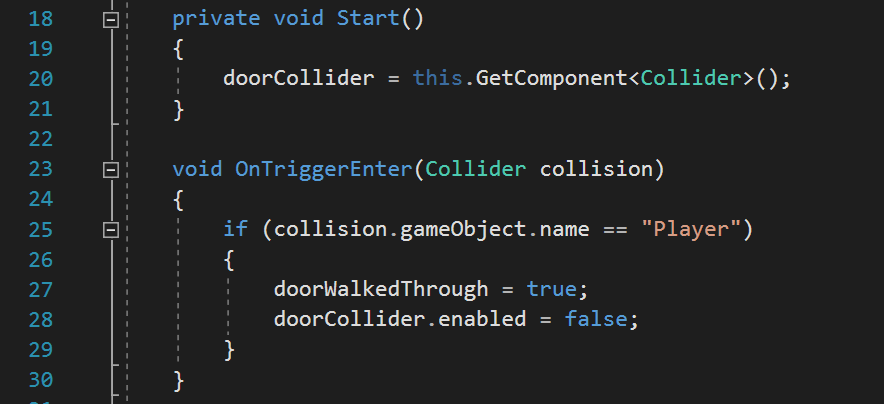
\includegraphics[width=1.0\linewidth]{DoorCode.png}
		\caption{A segment of the DoorState class that updates the door when the player walks through.}
		\label{image:DoorCode}
	\end{figure} 
	
	\subsubsection{Timer and Data Export}
	The second bot was to check whether the software could successfully export the necessary data to a .CSV file. This bot is the same as the door testing bot. Figure~\ref{image:ExportData} shows an example of the data exported from the game.  
	
	\begin{figure}[h]
		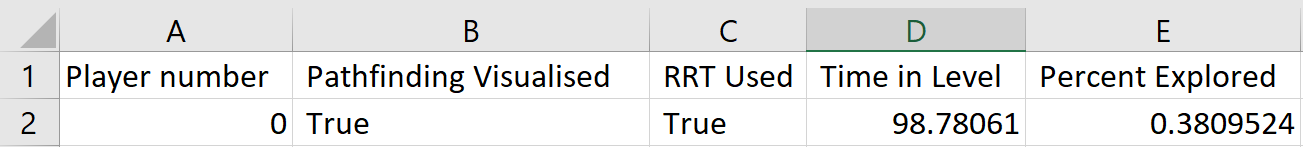
\includegraphics[width=1.0\linewidth]{ExportData.png}
		\caption{An example of the data exported from the game.}
		\label{image:ExportData}
	\end{figure} 
	
	\subsubsection{Visualisations}
	The final test was whether the path-finding visualisation worked as intended. This does not require a bot it can be seen tested by observing the scene in Unity. Figure~\ref{image:navmeshVisuals} shows the visualisation of the Unity navmesh working in the engine.  Figure~\ref{image:RRTVisuals} shows the visualisation of the RRT path-finding working in engine.
	
	\begin{figure}[h]
		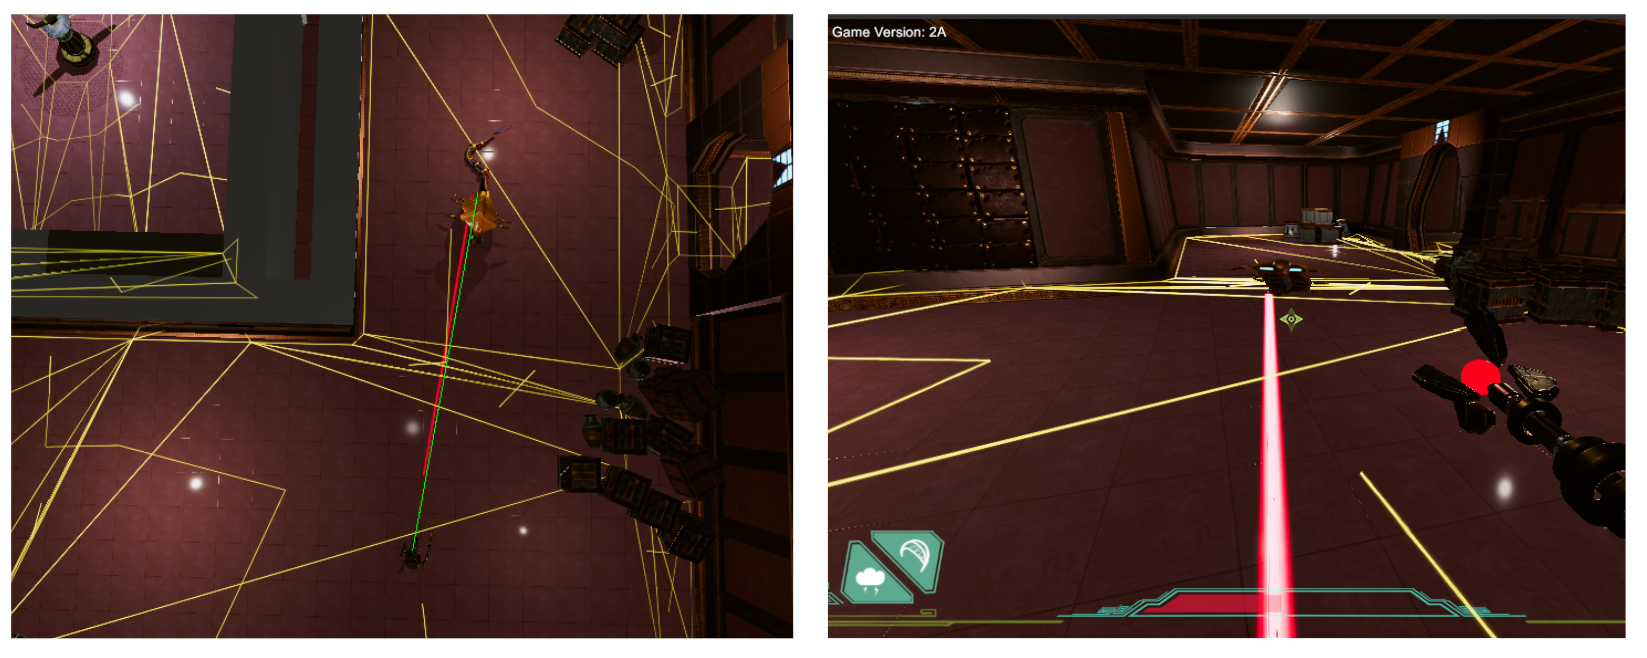
\includegraphics[width=1.0\linewidth]{NavmeshVis.png}
		\caption{The navmesh visualisations shown both in editor and in scene.}
		\label{image:navmeshVisuals}
	\end{figure}  
	
	
	\begin{figure}[h]
		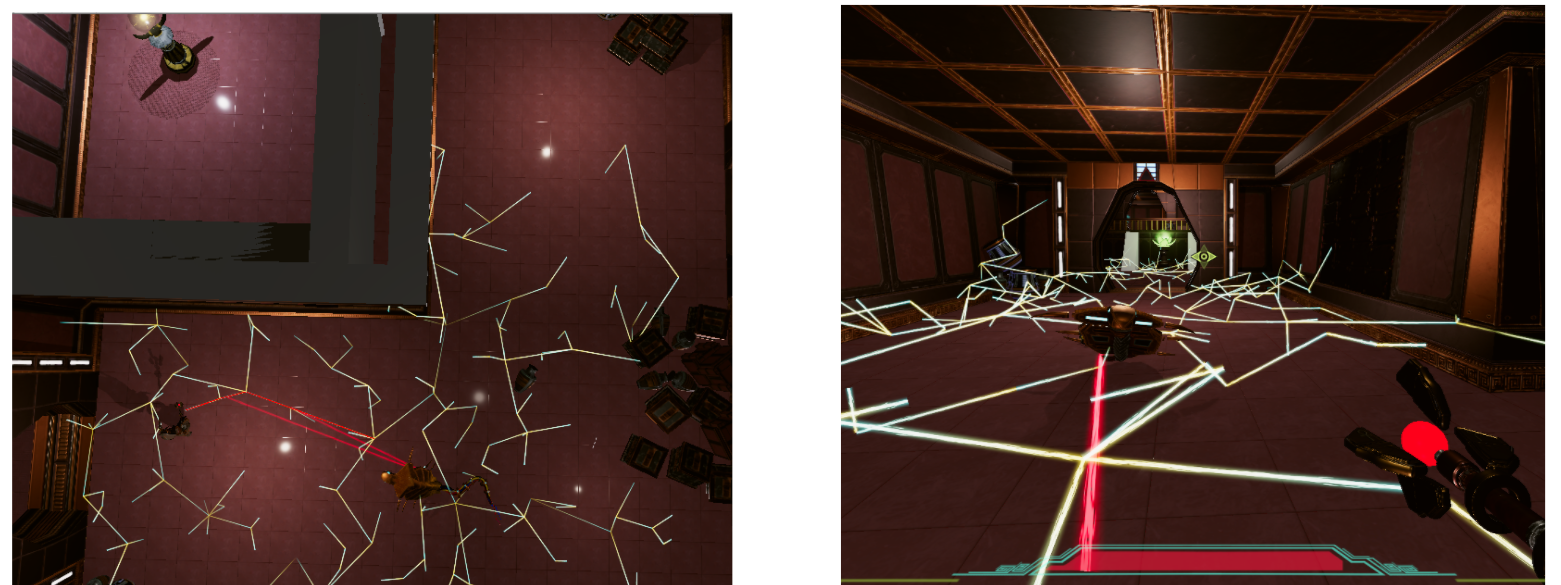
\includegraphics[width=1.0\linewidth]{RRTVis.png}
		\caption{The RRT visualisations shown both in editor and in scene.}
		\label{image:RRTVisuals}
	\end{figure}  
	
	\section{Data Collection and Filtering}  \label{datacollection}
	All the data used either came from the game's exported data or from the questionnaire.  Play-testing gave 107 datasets from 62 participants. However, as not all participants gave complete datasets 10 datasets have been removed leaving 97 datasets from 52 participants. 
	
	When the player dies in-game the game resets, this lead to a number of results having 0 percent explored and low play times. As these were not proper play-tests the 11 instances of this were removed from the dataset leaving 86 datasets. Many players also died within the first few minutes of playing, giving a play-test with a low time and exploration amount, the 34 instances of this were also removed from the dataset. Removing these left 52 datasets; one per player. There is a potential issue here where the player may not explore and area again if they have already explored it before dying. However, data from playthroughs where the player died in the first 5 minutes would have been more likely to have had an effect. 
	
	\section{Analysis and Interpretation} \label{Analysis}
	All the data analysis was conducted using R in R Studio. The results gathered can be seen in Table~\ref{StatsTable}.  Figure~\ref{image:RCor} shows an example of the code ran in R, it shows a correlation and a T-Test that have been run. 
	
	\begin{figure}[h]
		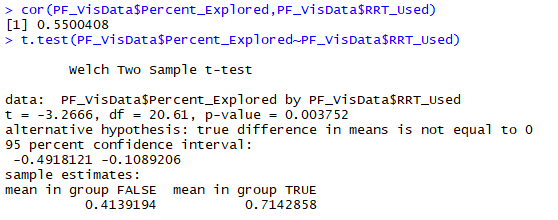
\includegraphics[width=1.0\linewidth]{RCor.png}
		\caption{An example of the R code used for calculating T-Tests and Correlations.}
		\label{image:RCor}
	\end{figure}  
	
	\begin{table*}[]
		\centering
		\caption{T-Test and Correlation Results}
		\label{StatsTable}
		\def\arraystretch{1.5}
		\begin{tabular}{|l|l|l|l|}
			\hline
			\textbf{Independent Variable }    &  \textbf{Dependent Variable } & \textbf{Correlation} & \textbf{T-Test - P Values}                   \\ \hline
			Visualising Path-finding& Percent Explored       & -0.1766742   & 0.2009            \\ \hline
			Visualised Path-Finding Methods    & Percent Explored         & 0.5500408    & 0.003752            \\ \hline
			RRT Used                & Percent Explored       & 0.2807048    & 0.04425           \\ \hline
			Non-Visualised RRT Use  & Percent Explored       & 0.2807048    & 0.04425           \\ \hline
			Visualised RRT          & Percent Explored       & 0.1697141    & 0.4229            \\ \hline
			Visualised NavMesh      & Percent Explored       & -0.4893995   & 0.01176           \\ \hline
			Visualised Path-finding & Time                   & 0.0002296794 & 0.9987            \\ \hline
			RRT Used                & Time                   & 0.06559258   & 0.6445            \\ \hline
			Visualised RRT          & Time                   & -0.0153404   & 0.9384            \\ \hline
			Visualised NavMesh      & Time                   & 0.001491802  & 0.9943            \\ \hline
			Visualised Path-finding & Understandable Visuals & 0.1627247    & 0.2731            \\ \hline
			RRT Used                & Understandable Visuals & 0.1910156    & 0.3341            \\ \hline
			Path-finding Visualised & Logical Enemy Movement & -0.2728879   & 0.06224           \\ \hline
			RRT Used                & Logical Enemy Movement & -0.01419318  & 0.9234            \\ \hline
			RRT Used                & Deaths                 & -0.2656382   & 0.05917           \\ \hline
			Visualised Path-finding & Deaths                 & 0.318452        & 0.01833        \\ \hline
		\end{tabular}
	\end{table*}
	
	Table~\ref{StatsTable} shows the correlations and P-Values from the T-Test results calculated using R.  In a majority of cases there was insufficient evidence to reject the null hypothesis. However, there are some cases that have a P-Value of less than 0.05 and are thus statistically significant. 
	
	\begin{figure}[h]
		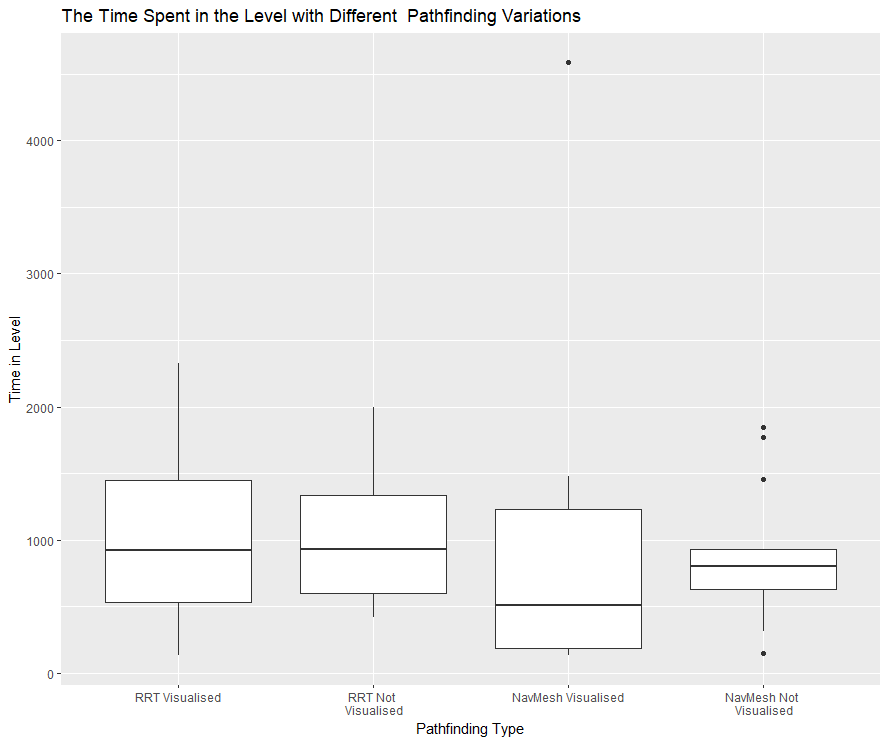
\includegraphics[width=1.0\linewidth]{GraphTime.png}
		\caption{Box and Whisker plot of the time spent in the level with the 4 game variations.}
		\label{graph:Time}
	\end{figure}  
	
	\begin{figure}[h]
		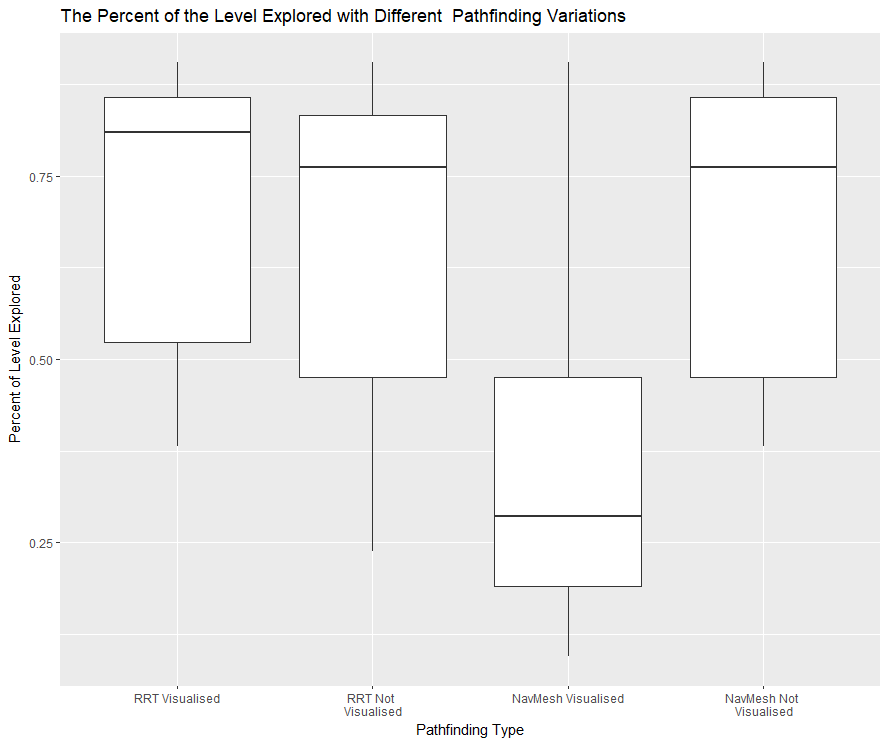
\includegraphics[width=1.0\linewidth]{GraphPercent.png}
		\caption{Box and Whisker plot of the percent of the level explored with the 4 game variations.}
		\label{graph:Percent}
	\end{figure}
	
	\subsection{RRT and the Percent of the Level Explored} \label{RRTExplore}
	The first significant correlation is a small positive correlation of 0.2807 between the percent of the level explored and the use RRT path-finding. This suggests that players explore more in the RRT variations.    
	
	
	The graph in figure~\ref{graph:Percent} shows that the percent explored between the two RRT variations are both close, with the not visualised variation being slightly lower. 
	
	There is no significant correlation between the RRT being visualised and the percent which would suggest that visualising the RRT does not affect the percent of the level explored. However, when just looking at visualised path-finding there is another significant correlation between the type of visualised path-finding used and the percent of the level explored. There is a strong positive correlation of 0.55 which again suggests that players explore more when RRT is used in comparison to NavMeshes. Another RRT related significant correlation is between non-visualised RRT and the percent explored which has a positive correlation of 0.281.  
	
	There is also no significant correlation between RRT use and the time spent in the level. This suggests while the players explored more when the RRT was used they do not spend more time in the level.  
	
	Some participants commented that they thought the RRT was leading somewhere and followed it through the level or went to it when they saw it.  However this only accounts for when the RRT is visualised. Another possibility is the RRT itself was spawned in a square and often did not fill a room which may encourage players to move around the edge of the room rather than down the middle they may have been more likely to find hidden doors increasing their exploration percentage.
	
	Another reason for this could be that in the play-testing software each RRT was limited to a single room as enemies could not follow players out of rooms this may have allowed them to avoid combat, or make combat faster, allowing them to explore more. 
	
	
	\subsection{NavMesh Visualisation and the Percent of the Level Explored}
	
	The second case was a negative correlation of -0.4894 between the percent explored and the NavMesh path-finding being visualised. This suggests that players explored less when the NavMesh was visualised.  As many play-testers were game development students using Unity they may have known what the visualisation was of the NavMesh was. This may have helped them find a quicker route through the level or lead them to avoid rooms with enemies in. Another reason could be that seeing the pathfinding showed them the possible pathways aiding them in finding a more direct path through the level
	
	\subsection{Visualised Path-Finding and Player Deaths}
	
	\begin{figure}[h]
		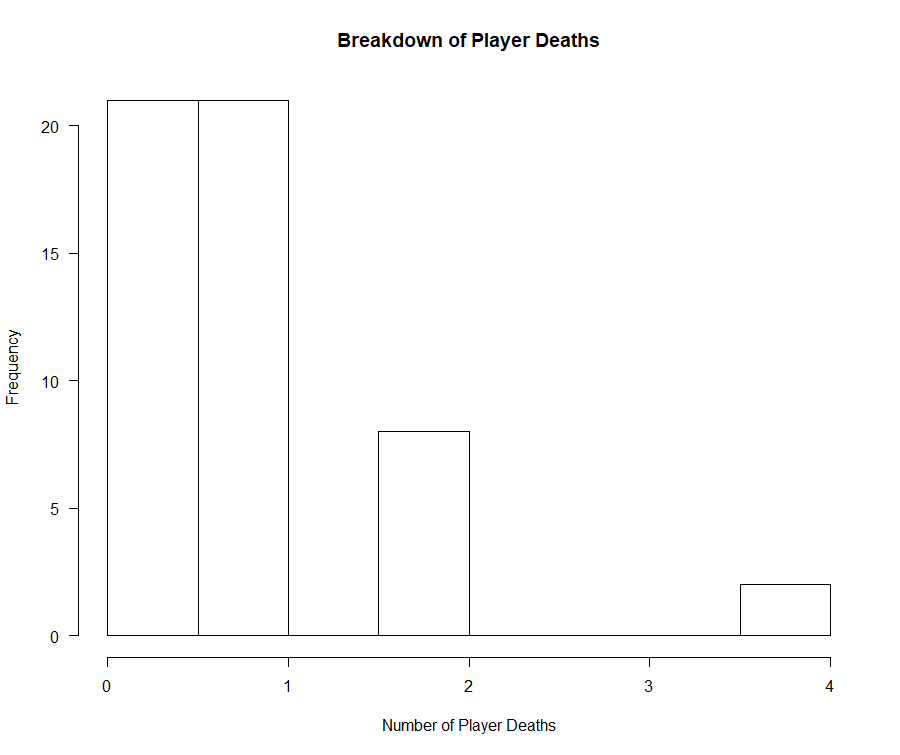
\includegraphics[width=1.0\linewidth]{DeathsHisto.png}
		\caption{Histogram of the frequency of the number of player deaths.}
		\label{graph:DeathsHisto}
	\end{figure}
	Another significant correlation is the positive correlation between the visualised path-finding and the number of player deaths. This means that players with the variations with visualised path-finding died more than players without it. One reason for this could be the player being distracted by the visualisation and therefore did not focus on enemies. 
	
	In the RRT variation, the tree visuals are only in areas where there are enemies, as some players claim to move to the RRT whenever they saw it they could have been more likely to find enemies than players without the visualisation.
	
	As can be seen in the graph in figure~\ref{graph:DeathsHisto} an equal number of players died 0 or 1 time. The one death could likely be due to the player not knowing how to play the game and learning and may have skewed the results. A smaller number of players died 2 or 4 times. 
	
	There is no correlation or statistical significance between the questionnaire data and the exported game data. This could potentially be due to poorly worded questions or players not understanding what the visualisation, as mentioned in more detail in section~\ref{PotentialIssues}. Many players claimed to understand the path-finding visualisation. However, the comments after playing suggested that they do not as many believed it was an aesthetic choice.
	
	Apart from the cases above, there was insufficient evidence to reject the null hypothesis......  This suggests that neither of the visualisations was more understandable than one another to the player. Also, neither the change in path-finding method or the visualisation affected the time spent in the level even when the percent explored increased.
	
	Figure~\ref{graph:Time} shows that the times for all four variations were close. However, unlike figure~\ref{graph:Percent} there are a number of outliers on the NavMesh variations. Firstly, on visualised NavMeshes, there was an outlier with over 4000 seconds spent in the level where a majority of the other play-tests for all four variations were under 2000. Finding this outlier in the play-test data showed that this player has a very high play time with a low exploration percent. As this was a remote player this suggests that the player just launched the level and left the game running without playing. Though the player did die so they may have made some attempt to play.
	
	
	\section{Potential Issues and Future Work} \label{PotentialIssues}
	While the methodology of the study worked, in this case, there were many areas that could be improved in future work to improve the quality of the data collected. This section identifies a number of weaknesses in this study and how they could be improved on. 
	
	\subsection{Play-testing Game} 
	A first potential issue with the play-testing is that the game was not specifically designed for this paper. While the game is a Metroidvania game with a focus on exploration a few participants noted the enemies in the game were very aggressive and a majority of players died at least once which could have affected their desire to explore. In a future study, a game would either be designed specifically for the play-testing or altered more to suit the study.  
	
	\subsection{Participants}
	Another issue with using the game `Gates of Amenti' is that many of the play-testers were game development students who have play-tested other levels of the game or seen the game trailer during the university show and tell day. This meant that they could have been looking for things they have previously seen in the trailer as opposed to exploring or being affected by the visualisation.
	
	In future work the player would also be selected randomly and from a larger pool of people. In this study, a majority of players were students studying a game development course.
	
	\subsection{Performance Issues}
	A second issue was the RRT variations of the game were more resource intensive to run than the Navmesh versions. This lead to a slight frame rate drop at the start of the game. 
	Many of the play-tests used Falmouth Games Academy's computers which were capable of running both versions well. However, some play-tests were done remotely and therefore their computer specification and therefore the performance of the game is unknown. In future studies, this would be combated by either doing all the play-tests in one location ensuring everyone uses similar computers or to expand on the games data collection to include the frame rate or expand the questionnaire to include player's computer specifications.     
	
	\subsection{Visualisation}    
	The visualisation itself was also potentially an issue as many players do not know what it was or they assumed it was part of the games aesthetic and ignored it. However, visualisation could still affect the player even if they do not understand the visualisation.  Many participants suggested they do not understand the RRT visualisation but the results still showed their exploration was effected. 
	
	However, as many players do not understand the visualisation it suggests that the questionnaire should have explained it to some extent to get better answers. This also combined with the issue of self-report bias as many players answered the questionnaire saying they understood the visualisation but when spoken to afterwards it became apparent they do not. 
	
	While the RRT visualisation worked as intended in future work an area to explore would be increasing the RRT size.  In this experiment, the RRT was performance heavy so in future work the RRT could be made more optimised and then the RRT can be increased in size and clustering could be used to filter the tree.
	
	\subsection{Collected Data}    
	While the data collected from the game was usable it could be refined to get more data that would allow for more in-depth analysis. For example, currently the game only records how many doors the player walks through, an improvement on this would be to record what doors they walked through to create heat maps and perform more statistical analysis to see whether players explore differently in the different game variations or if the player's died in similar locations.
	Another issue with the collected data is that with the questionnaire relied on players being honest. There could have been self-report bias where players gave different answers, for example, players were asked if they understood the visualisation and they were unlikely to admit to not understanding. This could be addressed in future work by relying more on in-game data and wording the questions differently.
	
	\subsection{Random Nature of RRT}
	As RRT randomly selects where to place its node each player would have a different RRT. This affects the enemy movement as it leads them to move in different ways. Also, some areas had clutter objects such as crates in them, if the path went through the crates they could be knocked over causing the enemy to have to move a different way and affecting how the player can move. 
	While A* always find the shortest path between two points it is very unlikely that players and enemies will be in the exact same spot and thus unlikely that players will get the same path from A*. 
	
	
	\section{Future Work} \label{FutureWork}
	The most unexpected significant results found in section~\ref{Analysis} was the NavMesh visualisation decreasing the percent of the level explored. Future research on this subject could research that in more detail to find a more definite reason for why that happened. 
	
	Also, as section~\ref{PotentialIssues} mentions there were issues with the game used in this study, as future research would require a different or more complete game it could also give interesting data to look at pathfinding in more complex environments and other game genres such as stealth games. 
	
	
	\section{Conclusion} 
	In conclusion, while the use of RRT is more frequent in robotics than digital games its use appears feasible in this project. Its past use in game design tools shows that clustering can make the output understandable to the user. However, the need of optimisations such as RRT* or the use of A* may arise to produce a shorter path or to find any path. 
	
	Visualisation and foregrounding of AI have been successfully used before suggesting that it can be used here. Finally, previous studies have looked at way-finding and player exploration. These suggest that environmental factors in digital environments do have some effect on player exploration.
	
	The results found that a number of significant results which means that to some extent the pathfinding method and visualisation effects the player's exploration in a level.  Like many of the papers reviewed in section~\ref{RelatedWork} this could be applied in game design. Level designers could take it into account what type of pathfinding will give the result they want as different results may be wanted for different genres or even different sections of the game. In this study visualising the pathfinding to the player often resulted in the player being unsure of what the visualisation was so more research may be required to use the visualisations in video games rather than just designing them.
	
	% references section
	\bibliographystyle{IEEEtran}
	\bibliography{references}
	
	% Appendices	
	\appendices
	\section{Acknowledgements}
	I would like to thank my project supervisor Dr. Edward Powley ....
	
	\section{First appendix: Reflective Report}
	%Appendices are optional. Delete or comment out this part if you do not need them.
	While I am pleased with the final paper I produced there are many parts to this paper and the software that I could have improved on. 
	
	\subsection{Play Testing}
	The first issue was play-testing I vastly underestimated how long this would take and left it too late. This lead to me struggling to get enough participants and resorting to getting more online. One way to address this in the future would be to run a larger pilot study. In this paper the pilot study consisted of 4 players, one for each variation. These all took around 20 minutes however in the actual study player took up to an hour. 
	
	\subsection{Data Collection}
	Another area that I would improve on in the future would be how the data is collected and what data is collected. One issue I had with the data collected in this experiment is that the data from the game and the data from the questionnaire were both separate 
	
	    * Play testing takes a long time
	    * Data logging needs to be better 
	
	\subsection{Time Management}
	
	
	% that's all folks
\end{document}
